\chapter{Results}
%\subsection{General results}
%
%After excluding faulty cameras we had TK cameras in total, 19 in the Control-group and 33 in the experiment group.
%A total of TK photos were taken, of whom TK contained photos of the species I've focused on in my study. Check table for more details.
%
%The species I've focused on was mainly night-active as displayed in the density plots \ref{fig:overlap}, (with the exception of squirrel). In other words, all of them experienced a white LED flash during night hours.
%(Caption: Figure is split up in periods with and without white LED flash. Night activity in the dashed curve highlights the times the species would have experienced the flash. "Carpet"-below the curves signifies datapoints of each "group".
%





\section{GLMM}


\subsection{All species}

As the control-group stayed unchanged through the whole study period, and was visited less than the other cameras, I expected there to be no trend over time (i.e. time.deploy $\approx 0$ in table \ref{tab:param}).
Any fluctuations in detection rates due to weekly (and ultimately seasonal) changes should be controlled for by the random effect-term for week of the year, leaving the control group as a representation of the baseline detection rate.
This held true for all the species in my analysis.

In general, the control-group had lower detection rates than the two treatment groups for all species (see table \ref{tab:param}).
However, for most species, the slopes of IR and LED are completely covered by the Control-group's confidence interval (CI), meaning that the differences are non-significant.


If there were any effect of the LED, the IR period should show a regression to the norm, ie. counteracting the effect of the LED.
Thus, if the LED had a negative slope along the time axis, the IR should have a positive slope.
Further, their respective main effects (ie. when time since deployment = 0) should correspond somewhat to the other factor's simple effect of when time since deployment is at maximum value (84 days).
Still, as time since deployment = 0 corresponds to the day of my visitation, my presence could skew that pattern to some extent.

The main effect of LED was positive for most species, although none responded significantly (table \ref{tab:param}).


% latex table generated in R 4.0.4 by xtable 1.8-4 package
% Fri Mar 26 20:35:32 2021
\centering
{\tiny\renewcommand{\arraystretch}{.8}
	\resizebox{!}{.35\paperheight}{%
		\begin{tabular}[c]{llrlcrrr}
  \toprule
Species & Parameter & Coefficient & SE & 95\% CI & z & p & SGPV \\ 
\midrule
Roe deer & Intercept & -2.85 & 0.38 & (-3.58, -2.11) & -7.57 & $<$ .001 & 0.00 \\ 
& Time & -0.05 & 0.02 & (-0.09, -0.01) & -2.24 & \textbf{0.025}  & \textit{1.00} \\ 
& IR & -0.26 & 0.44 & (-1.12,  0.60) & -0.59 & 0.557  & 0.14 \\ 
& wLED & -0.13 & 0.44 & (-0.99,  0.73) & -0.30 & 0.761  & 0.14 \\ 
& Time * IR & 0.02 & 0.03 & (-0.04,  0.08) & 0.71 & 0.476  & \textit{1.00} \\ 
& Time * wLED & $<$ 0.01 & 0.03 & (-0.05,  0.06) & 0.12 & 0.901  & \textit{1.00} \\ 
\midrule
Moose & Intercept & -4.15 & 0.30 & (-4.75, -3.56) & -13.75 & $<$ .001 & 0.00 \\ 
& Time & $<$ 0.01 & 0.05 & (-0.08,  0.10) & 0.14 & 0.890  & \textit{1.00} \\ 
& IR & 		-0.08 & 0.35 & (-0.77,  0.60) & -0.23 & 0.814  & 0.17 \\ 
& wLED & 	 0.30 & 0.34 & (-0.36,  0.97) & 0.89 & 0.373  & 0.18 \\ 
& Time * IR & 0.05 & 0.06 & (-0.06,  0.17) & 0.86 & 0.389  & 0.75 \\ 
& Time * wLED & $<$ 0.01 & 0.06 & (-0.12,  0.10) & -0.12 & 0.902  & \textit{1.00} \\ 
\midrule
Red deer & Intercept & -3.89 & 0.41 & (-4.69, -3.09) & -9.55 & $<$ .001 & 0.00 \\ 
& Time & -0.09 & 0.06 & (-0.21,  0.02) & -1.63 & 0.104  & 0.53 \\ 
& IR & $<$ 0.01 & 0.50 & (-0.99,  0.97) & -0.02 & 0.984  & 0.12 \\ 
& wLED & -0.69 & 0.53 & (-1.72,  0.35) & -1.30 & 0.192  & 0.12 \\ 
& Time * IR & 0.06 & 0.08 & (-0.09,  0.21) & 0.81 & 0.421  & 0.65 \\ 
& Time * wLED & 0.23 & 0.08 & ( 0.08,  0.38) & 2.96 & \textbf{0.003}  & 0.00 \\ 
\midrule
Badger & Intercept & -4.49 & 0.37 & (-5.22, -3.76) & -12.12 & $<$ .001 & 0.00 \\ 
& Time & 0.06 & 0.03 & ( 0.00,  0.13) & 1.85 & 0.064  & 0.82 \\ 
& IR & 0.17 & 0.39 & (-0.59,  0.93) & 0.44 & 0.657  & 0.16 \\ 
& wLED & 0.24 & 0.38 & (-0.51,  0.99) & 0.64 & 0.523  & 0.16 \\ 
& Time * IR & 0.01 & 0.04 & (-0.07,  0.09) & 0.27 & 0.784  & \textit{1.00} \\ 
& Time * wLED & $<$ 0.01 & 0.04 & (-0.07,  0.08) & 0.11 & 0.914  & \textit{1.00} \\ 
\midrule
Pine Marten & Intercept & -5.95 & 0.54 & (-7.02, -4.89) & -10.95 & $<$ .001 & 0.00 \\ 
& Time & 0.09 & 0.09 & (-0.09,  0.28) & 0.97 & 0.331  & 0.52 \\ 
& IR & 1.69 & 0.58 & ( 0.55,  2.82) & 2.92 & \textbf{0.004}  & 0.00 \\ 
& wLED & 0.76 & 0.61 & (-0.43,  1.95) & 1.25 & 0.210  & 0.10 \\ 
& Time * IR & -0.11 & 0.11 & (-0.32,  0.09) & -1.07 & 0.286  & 0.46 \\ 
& Time * wLED & 0.03 & 0.11 & (-0.18,  0.24) & 0.30 & 0.768  & 0.56 \\ 
\midrule
Red fox & Intercept & -3.44 & 0.26 & (-3.94, -2.94) & -13.40 & $<$ .001 & 0.00 \\ 
& Time & $<$ 0.01 & 0.03 & (-0.06,  0.05) & -0.02 & 0.985  & \textit{1.00} \\ 
& IR & 0.03 & 0.32 & (-0.59,  0.65) & 0.09 & 0.926  & 0.19 \\ 
& wLED & 0.18 & 0.31 & (-0.44,  0.79) & 0.56 & 0.574  & 0.19 \\ 
& Time * IR & $<$ 0.01 & 0.04 & (-0.08,  0.07) & -0.06 & 0.949  & \textit{1.00} \\ 
& Time * wLED & -0.01 & 0.04 & (-0.08,  0.06) & -0.30 & 0.763  & \textit{1.00} \\ 
\midrule
Lynx & Intercept & -4.82 & 0.58 & (-5.96, -3.67) & -8.24 & $<$ .001 & 0.00 \\ 
& Time & -0.22 & 0.14 & (-0.49,  0.05) & -1.58 & 0.113  & 0.24 \\ 
& IR & -0.20 & 0.72 & (-1.61,  1.21) & -0.28 & 0.781  & 0.08 \\ 
& wLED & 0.15 & 0.72 & (-1.26,  1.55) & 0.20 & 0.839  & 0.08 \\ 
& Time * IR & 0.25 & 0.16 & (-0.07,  0.57) & 1.53 & 0.127  & 0.22 \\ 
& Time * wLED & 0.26 & 0.16 & (-0.06,  0.58) & 1.59 & 0.112  & 0.20 \\ 
\midrule
Hare & Intercept & -3.91 & 0.36 & (-4.61, -3.21) & -10.94 & $<$ .001 & 0.00 \\ 
& Time & 0.04 & 0.03 & (-0.03,  0.10) & 1.12 & 0.263  & \textit{1.00} \\ 
& IR & 0.38 & 0.42 & (-0.44,  1.21) & 0.91 & 0.363  & 0.14 \\ 
& wLED & 0.25 & 0.42 & (-0.58,  1.08) & 0.59 & 0.555  & 0.14 \\ 
& Time * IR & -0.05 & 0.04 & (-0.13,  0.03) & -1.26 & 0.209  & 0.88 \\ 
& Time * wLED & $<$ 0.01 & 0.04 & (-0.08,  0.08) & 0.03 & 0.975  & \textit{1.00} \\ 
\midrule
Red squirrel & Intercept & -4.82 & 0.41 & (-5.63, -4.00) & -11.63 & $<$ .001 & 0.00 \\ 
& Time & 0.08 & 0.05 & (-0.01,  0.18) & 1.67 & 0.095  & 0.62 \\ 
& IR & 0.91 & 0.47 & (-0.02,  1.83) & 1.93 & 0.054  & 0.00 \\ 
& wLED & 0.61 & 0.48 & (-0.32,  1.54) & 1.28 & 0.201  & 0.13 \\ 
& Time * IR & -0.17 & 0.06 & (-0.29, -0.05) & -2.85 & \textbf{0.004}  & 0.13 \\ 
& Time * wLED & -0.02 & 0.06 & (-0.13,  0.10) & -0.29 & 0.771  & 0.92 \\ 
   \bottomrule
\end{tabular}}}

	%Caption outside the .tex-file or else it would be deleted every time I update the parameter-table
\caption[Standardised model parameters]%
{\label{tab:param} Standardised model parameters \par \small Results of generalised linear mixed effect models on detection rate of species at 56 different locations in south-eastern Norway, with three different treatment levels; period with only IR camera (flash[IR]), period with additional white LED camera (flash[LED]) and site unchanged through the whole study period (flash[Control]). Random effects are location ID and week of year. Standardised parameters were obtained by fitting the model on a standardised version of the dataset. 95\% Confidence Intervals and p-values were computed using the Wald approximation.}

\end{table} % må inn og fjerne end{table} kvar gong tabellen oppdaterest!

 
%

\begin{figure}
		\begin{subfigure}{.5\textwidth}
		  \centering
		  	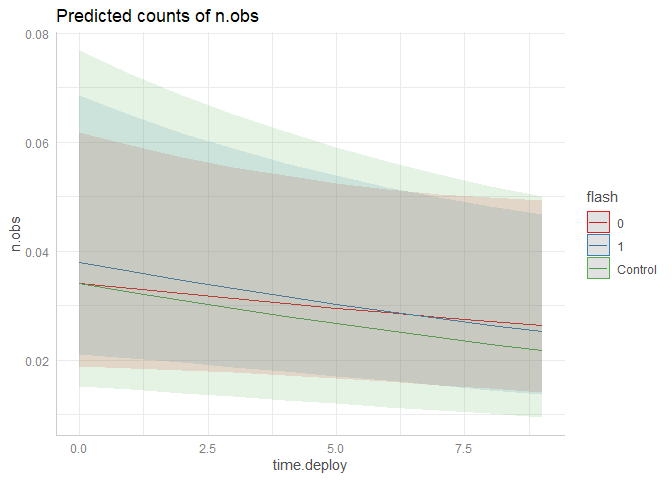
\includegraphics[width=.8\linewidth]{../R/glmm_sp_files/figure-gfm/raadyr-C-report-1.png}
		  \caption{Roe deer}
		  	\label{fig:glmm_raa}
	\end{subfigure}
		\begin{subfigure}{.5\textwidth}
		  \centering
		  	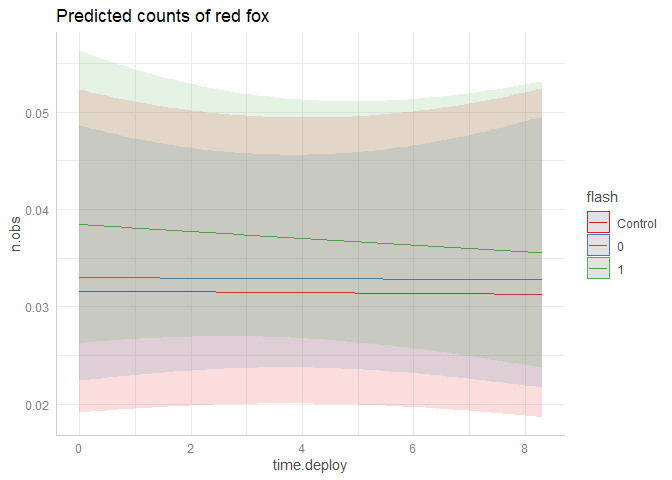
\includegraphics[width=.8\linewidth]{../R/glmm_sp_files/figure-gfm/rev-report-1.png}
		  \caption{Red fox}
		  	\label{fig:glmm_rev}
	\end{subfigure}
		\begin{subfigure}{.5\textwidth}
		  \centering
		  	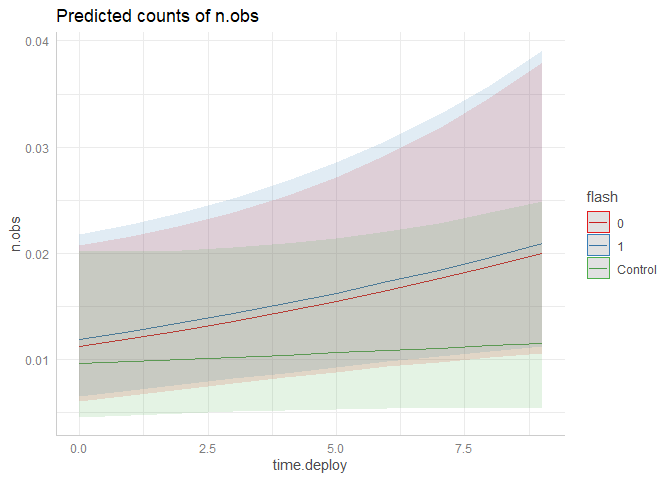
\includegraphics[width=.8\linewidth]{../R/glmm_sp_files/figure-gfm/grevling-report-1.png}
		  \caption{Badger}
		  	\label{fig:glmm_grvl}
	\end{subfigure}
		\begin{subfigure}{.5\textwidth}
		  \centering
		  	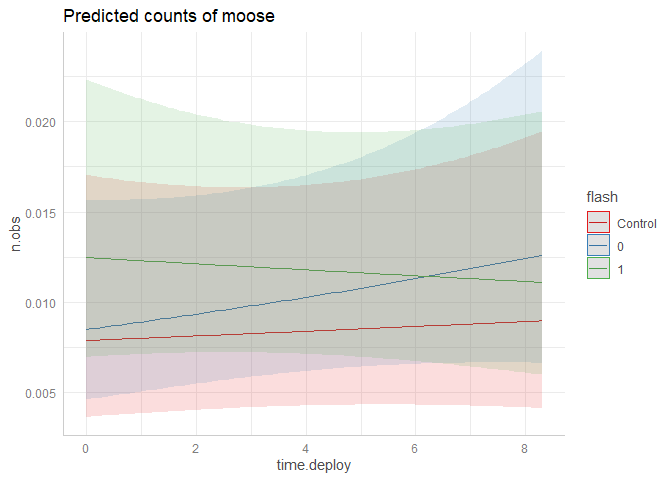
\includegraphics[width=.8\linewidth]{../R/glmm_sp_files/figure-gfm/elg-report-1.png}
		  \caption{Moose}
		  	\label{fig:glmm_elg}
	\end{subfigure}
		\begin{subfigure}{.5\textwidth}
		  \centering
		  	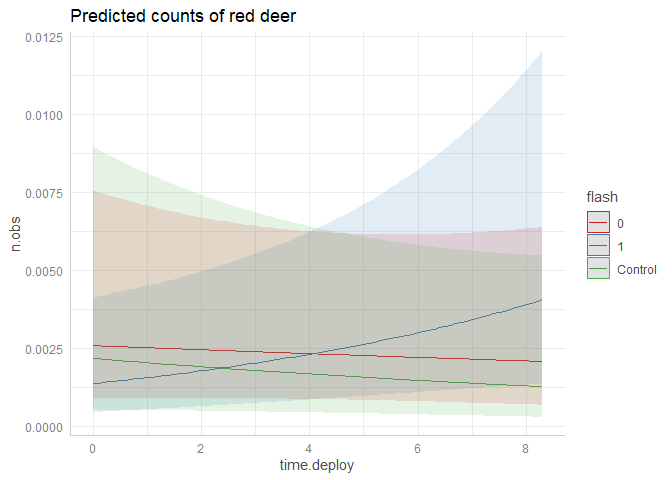
\includegraphics[width=.8\linewidth]{../R/glmm_sp_files/figure-gfm/hjort-report-1.png}
		  \caption{Red deer}
		  	\label{fig:glmm_hjort}
	\end{subfigure}
		\begin{subfigure}{.5\textwidth}
		  \centering
		  	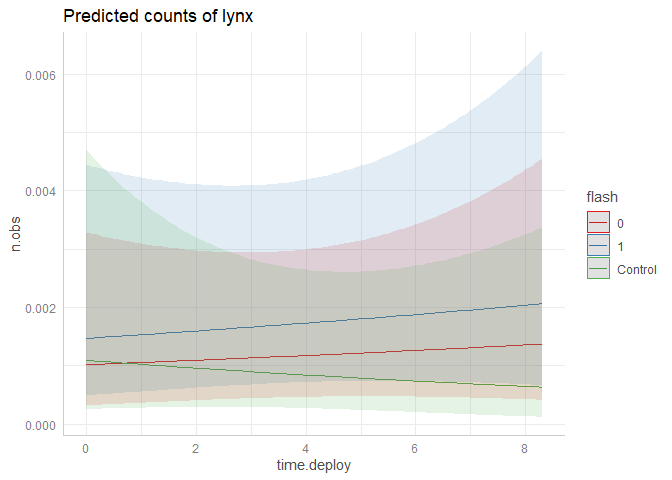
\includegraphics[width=.8\linewidth]{../R/glmm_sp_files/figure-gfm/gaupe-report-1.png}
		  \caption{Lynx}
		  	\label{fig:glmm_gaup}
	\end{subfigure}
		\caption{Fitted GLMM model to each species}
	\label{fig:glmm_sp}
\end{figure}



\begin{figure}
		\begin{subfigure}{.4\textwidth}
		  \centering
	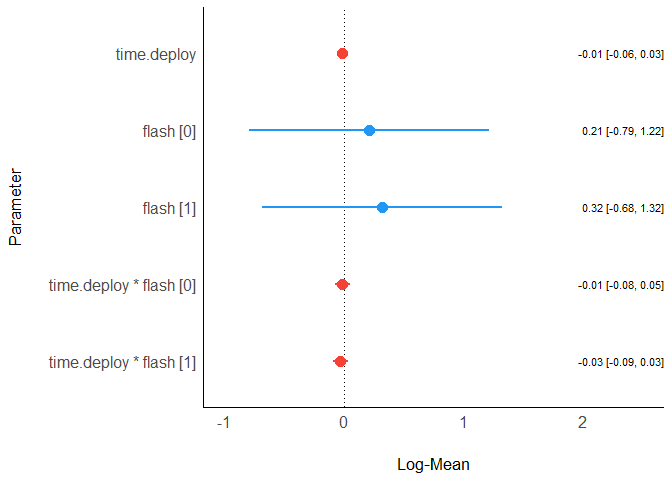
\includegraphics[scale=.4]{../R/glmm_sp_files/figure-gfm/parameters-1.png}
\caption{Intercept included}
		\label{fig:para_raa1}
	\end{subfigure}
		\begin{subfigure}{.4\textwidth}
		  \centering
	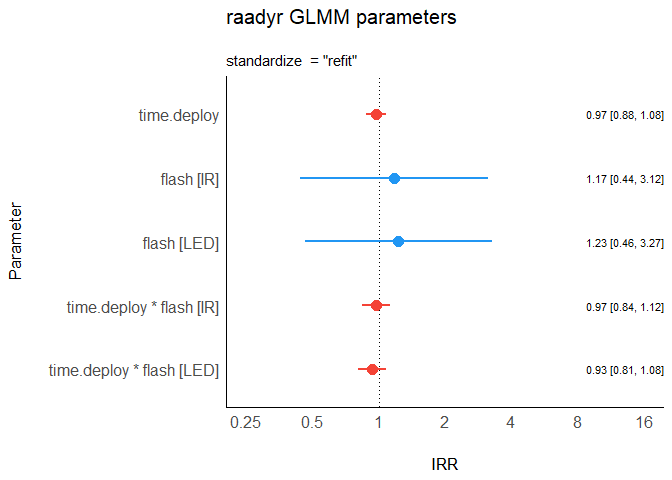
\includegraphics[scale=.4]{../R/glmm_sp_files/figure-gfm/parameters-2.png}
\caption{with values printed}
		\label{fig:para_raa2}
	\end{subfigure}
		\begin{subfigure}{.8\textwidth}
		  \centering
	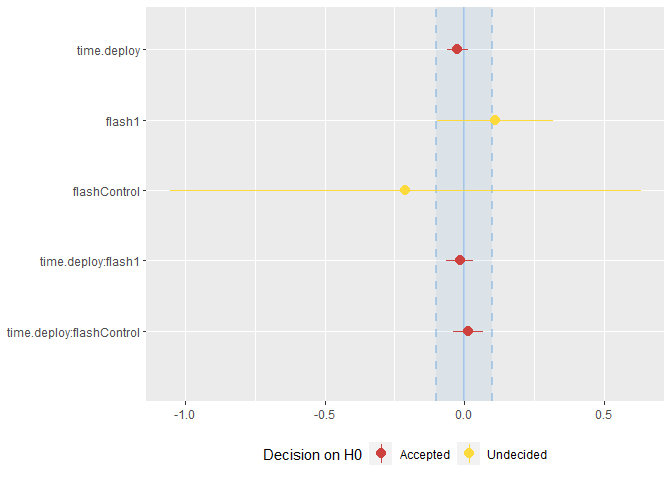
\includegraphics[scale=1]{../R/glmm_sp_files/figure-gfm/parameters-3.png}
\caption{Equivalence test}
		\label{fig:para_raa3}
	\end{subfigure}
		\caption{Visualising model parameters}
	\label{fig:para_sp}
\end{figure}




% On interpretation of relative risks / Incidence rate ratios (which is pretty similar to the coxph)
%https://sphweb.bumc.bu.edu/otlt/mph-modules/ep/ep713_association/ep713_association3.html

\clearpage %to force the insertion of parameters table

\subsection{Roe deer}

\begin{figure}
\centering
	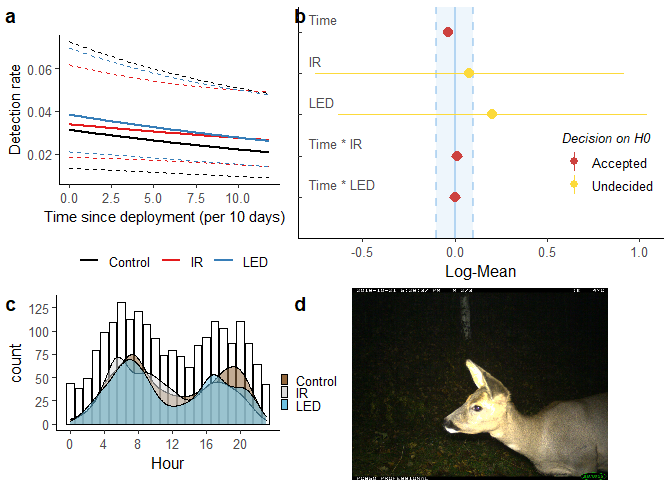
\includegraphics[scale=.9]{../R/glmm_sp_files/figure-html/parameters-1.png}
\caption[Roe deer]%
{Roe deer \par \small a) The predicted detection rate of roe deer for each level of the flash-variable. Confidence intervals (CI) represented by dotted lines.\\
b) Model parameters presented in an equivalence test. ROPE is set to $\pm$0.1 Log-Mean, $CI =1 - 2\times \alpha$.\\ 
c) Bars represent the raw count of total roe deer detections per hour of the day, and density curves show the overall pattern for each group.\\
d) LED-CT photograph of a roe deer. The deer passed the camera repeatedly and often stopped in front of the flashing light}\label{fig:raadyr}
\end{figure}


For roe deer, the model explaining variation in detection rate has a substantial explanatory power (conditional R2 = 0.45), but the part related to the fixed effects alone (marginal R2) is just 0.002.
In other words, most of the explained variation in detection rate is due to seasonal changes and variation between the different camera sites captured in the random terms.

The main effect of the white LED periods were non-significantly positive (flash[LED] in table \ref{tab:param}) compared to the control-group (Intercept).
The same is true for the IR periods, although to a slightly lower extent.
However, along the time since deployment-axis (time.deploy $\ast$ flash [LED]) there was a negative effect, to the extent that after two months the mean detection rate sank below that of the IR periods (see figure \ref{fig:raadyr}a).
Nevertheless, the confidence intervals (CI) of both white LED and IR periods almost completely overlap, and hence, are not significantly different.


When a parameter is within the ROPE in an equivalence test, it signifies that the difference from the Log-mean, and the variance of the parameter, is low enough that we can accept H0, rather than just fail to reject it.

According to this test, white LED is different enough that we cannot conclude on it’s main effect, but it’s trend over time (Time * LED) is practically equivalent to H0. 
In other words, the equivalence test suggests that there is no significant difference in the long run, but there might be an increase in detections right after the day of deployment.
However, the increase could also result from inhereting a slightly higher detection rate from the IR periods \emph{if} there truly is a negative effect of the white LED over long periods of time.



\newpage
\subsection{Red fox}

\begin{figure}
		  \centering
	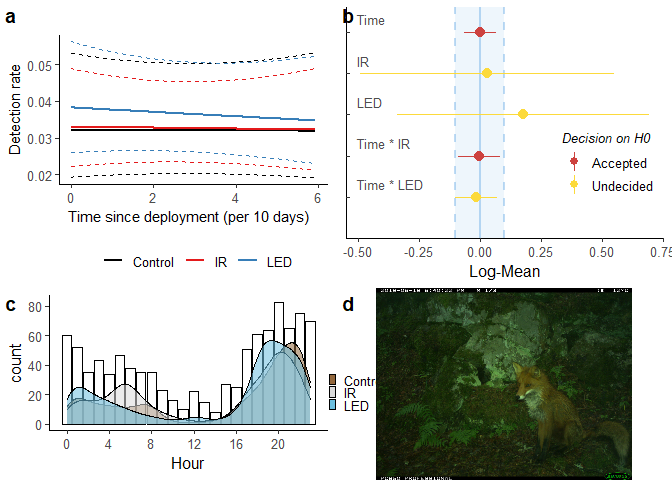
\includegraphics[scale=.9]{../R/glmm_sp_files/figure-html/rev2-1.png}
\caption[Red fox]%
{Red fox \par \small a) The predicted detection rate of red foxes for each level of the flash-variable. Confidence intervals (CI) represented by dotted lines.\\ 
b) Model parameters presented in an equivalence test. ROPE is set to $\pm$0.1 Log-Mean, $CI =1 - 2\times \alpha$.\\ 
c) Bars represent the raw count of total fox detections per hour of the day, and density curves show the overall pattern for each group.\\
d) LED-CT photograph of a red fox. The fox stopped in front of the flashing camera and waited for a following individual before they continued.}\label{fig:rev}
\end{figure}


For red fox, the model explaining variation in detection rate has a moderate explanatory power (conditional R2 = 0.19), and the part related to the fixed effects alone (marginal R2) is just 0.001. 


The main effect of the white LED periods were non-significantly positive (flash[LED] in table \ref{tab:param}) compared to the IR- and control-periods (flash[IR];Intercept) .
However, along the time since deployment-axis (time.deploy $\ast$ flash [LED]) there was a negative effect, to the extent that after two months the mean detection rate sank below that of the IR periods (see figure \ref{fig:raadyr}a).
Nevertheless, the confidence intervals (CI) of both white LED and IR periods almost completely overlap, and hence, are not significantly different.


\newpage
\subsection{Badger}

\begin{figure}
		  \centering
	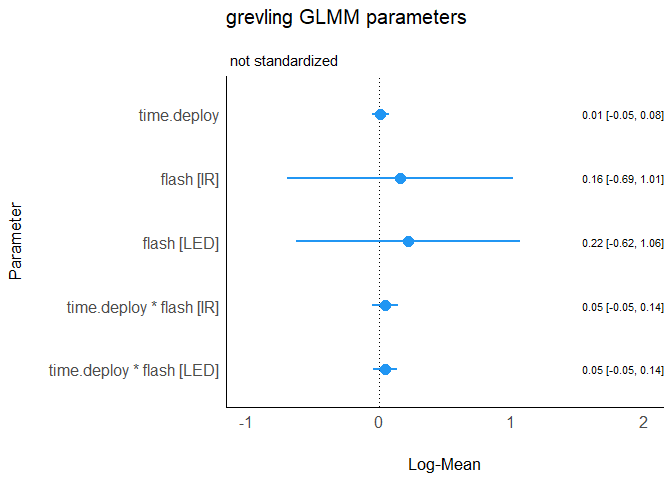
\includegraphics[scale=.9]{../R/glmm_sp_files/figure-html/grevling2-1.png}
\caption[Badger]%
{Badger \par \small a) The predicted detection rate of badgers for each level of the flash-variable. Confidence intervals (CI) represented by dotted lines.\\ 
b) Model parameters presented in an equivalence test. ROPE is set to $\pm$0.1 Log-Mean, $CI =1 - 2\times \alpha$.\\ 
c) Bars represent the raw count of total badger detections per hour of the day, and density curves show the overall pattern for each group.\\ 
d) LED-CT photograph of a badger. DESCRIPT}\label{fig:grevling}
\end{figure}

For badger, the model explaining variation in detection rate has a substantial explanatory power (conditional R2 = 0.42), but the part related to the fixed effects alone (marginal R2) is just 0.006.




\newpage
\subsection{Moose}

\begin{figure}
		  \centering
	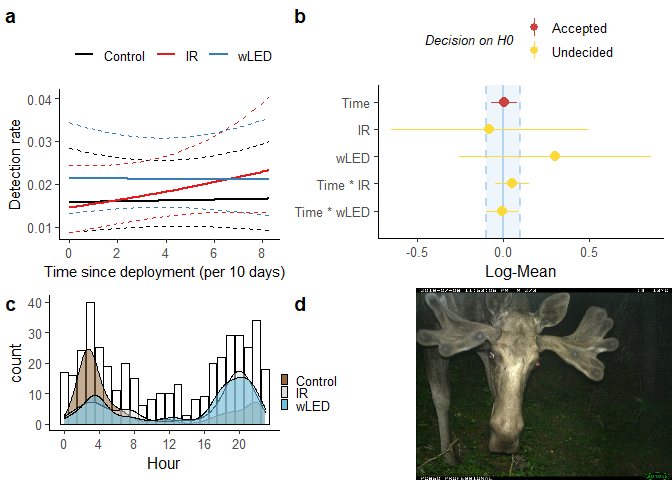
\includegraphics[scale=.9]{../R/glmm_sp_files/figure-html/elg2-1.png}
\caption[Moose]%
{Moose \par \small a) The predicted detection rate of moose for each level of the flash-variable. Confidence intervals (CI) represented by dotted lines.\\
b) Model parameters presented in an equivalence test. ROPE is set to $\pm$0.1 Log-Mean, $CI =1 - 2\times \alpha$.\\
c) Bars represent the raw count of total detections per hour of the day, and density curves show the overall pattern for each group\\
d) LED-CT photograph of a Moose. DESCRIPT}\label{fig:elg}
\end{figure}


\newpage
\subsection{Red deer}

\begin{figure}
		  \centering
	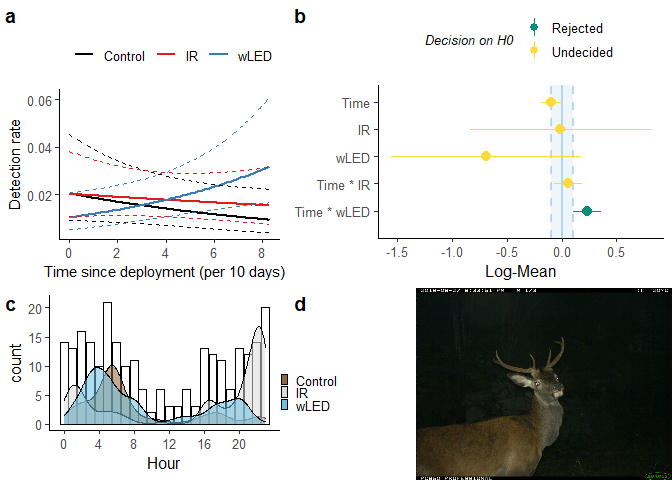
\includegraphics[scale=.9]{../R/glmm_sp_files/figure-html/hjort2-1.png}
\caption[Red deer]%
{Red deer \par \small a) The predicted detection rate of red deer for each level of the flash-variable. Confidence intervals (CI) represented by dotted lines.\\
b) Model parameters presented in an equivalence test. ROPE is set to $\pm$0.1 Log-Mean, $CI =1 - 2\times \alpha$.\\ 
c) Bars represent the raw count of total Red deer detections per hour of the day, and density curves show the overall pattern for each group.\\ 
d) LED-CT photograph of a red deer. DESCRIPT}\label{fig:hjort}
\end{figure}



\newpage
\subsection{Lynx}

\begin{figure}
		  \centering
	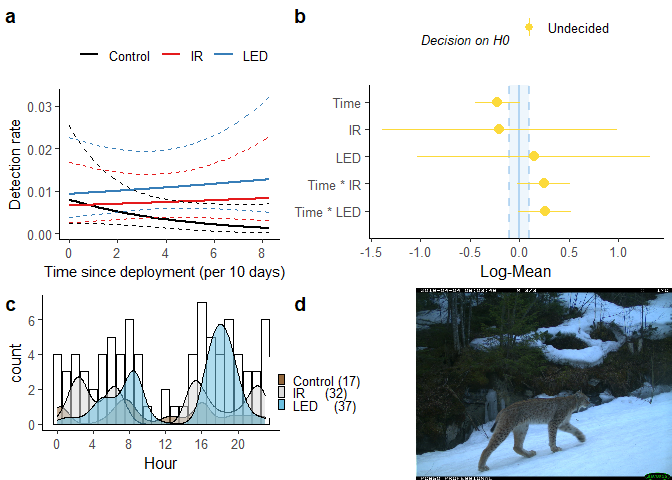
\includegraphics[scale=.9]{../R/glmm_sp_files/figure-html/gaupe2-1.png}
\caption[Lynx]%
{Lynx \par \small a) The predicted detection rate of lynx for each level of the flash-variable. Confidence intervals (CI) represented by dotted lines.\\ 
b) Model parameters presented in an equivalence test. ROPE is set to $\pm$0.1 Log-Mean, $CI =1 - 2\times \alpha$.\\ 
c) Bars represent the raw count of total lynx detections per hour of the day, and density curves show the overall pattern for each group.\\ 
d) LED-CT photograph of a lynx. DESCRIPT}\label{fig:gaupe}
\end{figure}





\newpage
\subsection{Hare}

\begin{figure}
		  \centering
	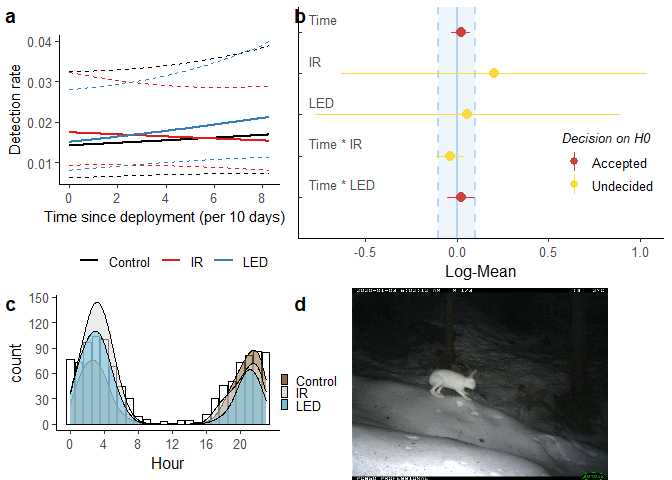
\includegraphics[scale=.9]{../R/glmm_sp_files/figure-html/hare2-1.png}
\caption[Hare]%
{Hare \par \small a) The predicted detection rate of hares for each level of the flash-variable. Confidence intervals (CI) represented by dotted lines.\\ 
b) Model parameters presented in an equivalence test. ROPE is set to $\pm$0.1 Log-Mean, $CI =1 - 2\times \alpha$.\\ 
c) Bars represent the raw count of total hare detections per hour of the day, and density curves show the overall pattern for each group.\\ 
d) LED-CT photograph of a hare. DESCRIPT}\label{fig:hare}
\end{figure}






\newpage
\subsection{Pine marten}

\begin{figure}
		  \centering
	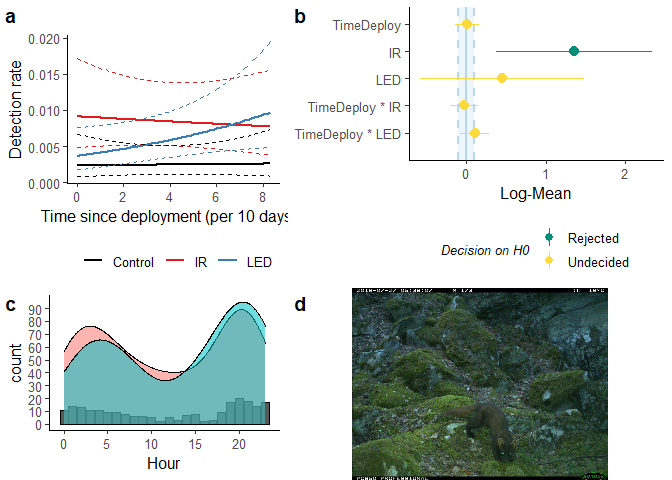
\includegraphics[scale=.9]{../R/glmm_sp_files/figure-html/maar2-1.png}
\caption[Pine marten]%
{Pine marten \par \small a) The predicted detection rate of pine martens for each level of the flash-variable. Confidence intervals (CI) represented by dotted lines.\\ 
b) Model parameters presented in an equivalence test. ROPE is set to $\pm$0.1 Log-Mean, $CI =1 - 2\times \alpha$.\\ 
c) Bars represent the raw count of total pine marten detections per hour of the day, and density curves show the overall pattern for each group.\\ 
d) LED-CT photograph of a pine marten. DESCRIPT}\label{fig:maar}
\end{figure}






\newpage
\subsection{Red squirrel}

\begin{figure}
		  \centering
	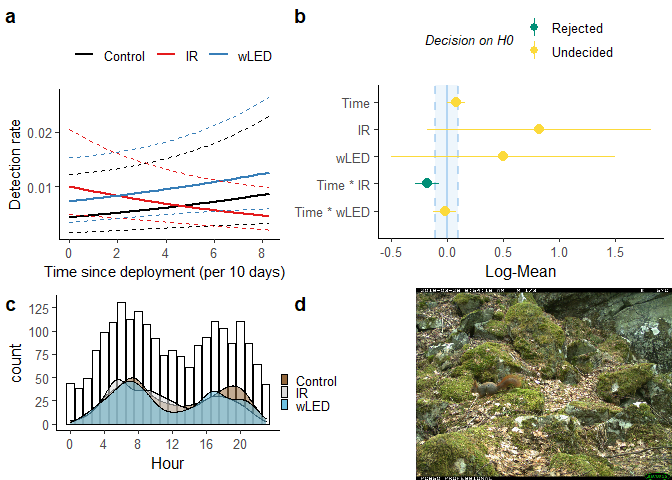
\includegraphics[scale=.9]{../R/glmm_sp_files/figure-html/ekorn2-1.png}
\caption[Red squirrel]%
{Red squirrel \par \small a) The predicted detection rate of squirrels for each level of the flash-variable. Confidence intervals (CI) represented by dotted lines.\\ 
b) Model parameters presented in an equivalence test. ROPE is set to $\pm$0.1 Log-Mean, $CI =1 - 2\times \alpha$.\\ 
c) Bars represent the raw count of total squirrel detections per hour of the day, and density curves show the overall pattern for each group.\\ 
d) LED-CT photograph of a squirrel. DESCRIPT}\label{fig:s}
\end{figure}

The model for red squirrel failed to converge, and therefore the p-values should be disregarded. 

Still, it is interesting to see the IR and LED-slopes crossing each other. Looking at the density plot, one would not expect that most squirrels were flashed by the white LED particularly often, as most detections are during the day.



%\subsection{CPH mixed effect}
%n.obs ~ time.deploy + flash*species + random.eff






